%\documentclass[sigchi]{acmart}
\documentclass[manuscript,review,anonymous]{acmart}

\input{sections/_preamble.tex}
\input{sections/_template_args.tex}
\input{sections/_command.tex}
% \usepackage{multirow}
\usepackage{multicol}
\usepackage{float}
\usepackage{amssymb}

\usepackage{tikz}
\usetikzlibrary{shapes, arrows, positioning}
\usepackage{orcidlink}

% Define custom colors
\definecolor{preprocessfill}{HTML}{e1d5e7}
\definecolor{preprocessdraw}{HTML}{9673a6}
\definecolor{featureprocfill}{HTML}{ffe6cc}
\definecolor{featureprocdraw}{HTML}{d79b00}
\definecolor{featureextfill}{HTML}{dae8fc}
\definecolor{featureextdraw}{HTML}{6c8ebf}
\definecolor{featureencfill}{HTML}{d5e8d4}
\definecolor{featureencdraw}{HTML}{82b366}
\definecolor{featurefusfill}{HTML}{f8cecc}
\definecolor{featurefusdraw}{HTML}{b85450}
\definecolor{featuredecfill}{HTML}{d5e8d4}
\definecolor{featuredecdraw}{HTML}{82b366}
\definecolor{renderfill}{HTML}{fff2cc}
\definecolor{renderdraw}{HTML}{d6b656}
\definecolor{modelfill}{HTML}{f5f5f5}

%%
%% end of the preamble, start of the body of the document source.
\begin{document}



%%
%% The "title" command has an optional parameter,
%% allowing the author to define a "short title" to be used in page headers.
\title{DeepGesture: A conversational gesture synthesis system based on emotions and semantics}

%%
%% Authors.
\input{sections/0_authors.tex}

%%
%% The abstract is a short summary of the work to be presented in the
%% article.

%    Gesture generation is a pivotal aspect of multimodal communication systems, enhancing the naturalness and contextuality of human-machine interactions. While significant progress has been made in this field for various languages, gesture generation tailored specifically for Vietnamese remains underexplored. This paper introduces \textbf{DeepGesture}, a diffusion-based gesture generation model base on emotions and semantics.

%Key to bunGesture is its adoption of diffusion-based gesture generation, integrating advanced Vietnamese language models like PhoBERT and the VnCoreNLP toolkit. Additionally, bunGesture employs a fine-tuned Vietnamese version of WaveLM, trained on a custom Vietnamese audio dataset.
%
%This work emphasizes the importance of language-specific adaptations in gesture generation systems and opens avenues for similar research in other languages.


\begin{abstract}
	Along with the explosion of large language models, improvements in speech synthesis, advancements in hardware, and the evolution of computer graphics, the current bottleneck in creating digital humans lies in generating character movements that correspond naturally to text or speech inputs.
	
	In this work, we present \textbf{DeepGesture}, a diffusion-based gesture synthesis framework for generating expressive co-speech gestures conditioned on multimodal signals—text, speech, emotion, and seed motion. Built upon the DiffuseStyleGesture model, DeepGesture introduces novel architectural enhancements that improve semantic alignment and emotional expressiveness in generated gestures. Specifically, we integrate fast text transcriptions as semantic conditioning and implement emotion-guided classifier-free diffusion to support controllable gesture generation across affective states. A lightweight Transformer backbone combines  and cross-local attention for effective feature fusion of heterogeneous modalities. To visualize results, we implement a full rendering pipeline in Unity based on BVH output from the model. Evaluation on the ZeroEGGS dataset shows that DeepGesture produces gestures with improved human-likeness and contextual appropriateness, outperforming baselines on Mean Opinion Score and Fréchet Gesture Distance metrics. Our system supports interpolation between emotional states and demonstrates generalization to out-of-distribution speech, including synthetic voices—marking a step forward toward fully multimodal, emotionally aware digital humans.
\end{abstract}



%%
%% Article info.
\input{sections/0_article_info.tex}

%%
%% Keywords. The author(s) should pick words that accurately describe
%% the work being presented. Separate the keywords with commas.
\keywords{co-speech gesture synthesis, gesture generation, character animation, diffusion model, neural generative model}


%% A "teaser" image appears between the author and affiliation
%% information and the body of the document, and typically spans the
%% page.
\begin{teaserfigure}
	\centering
  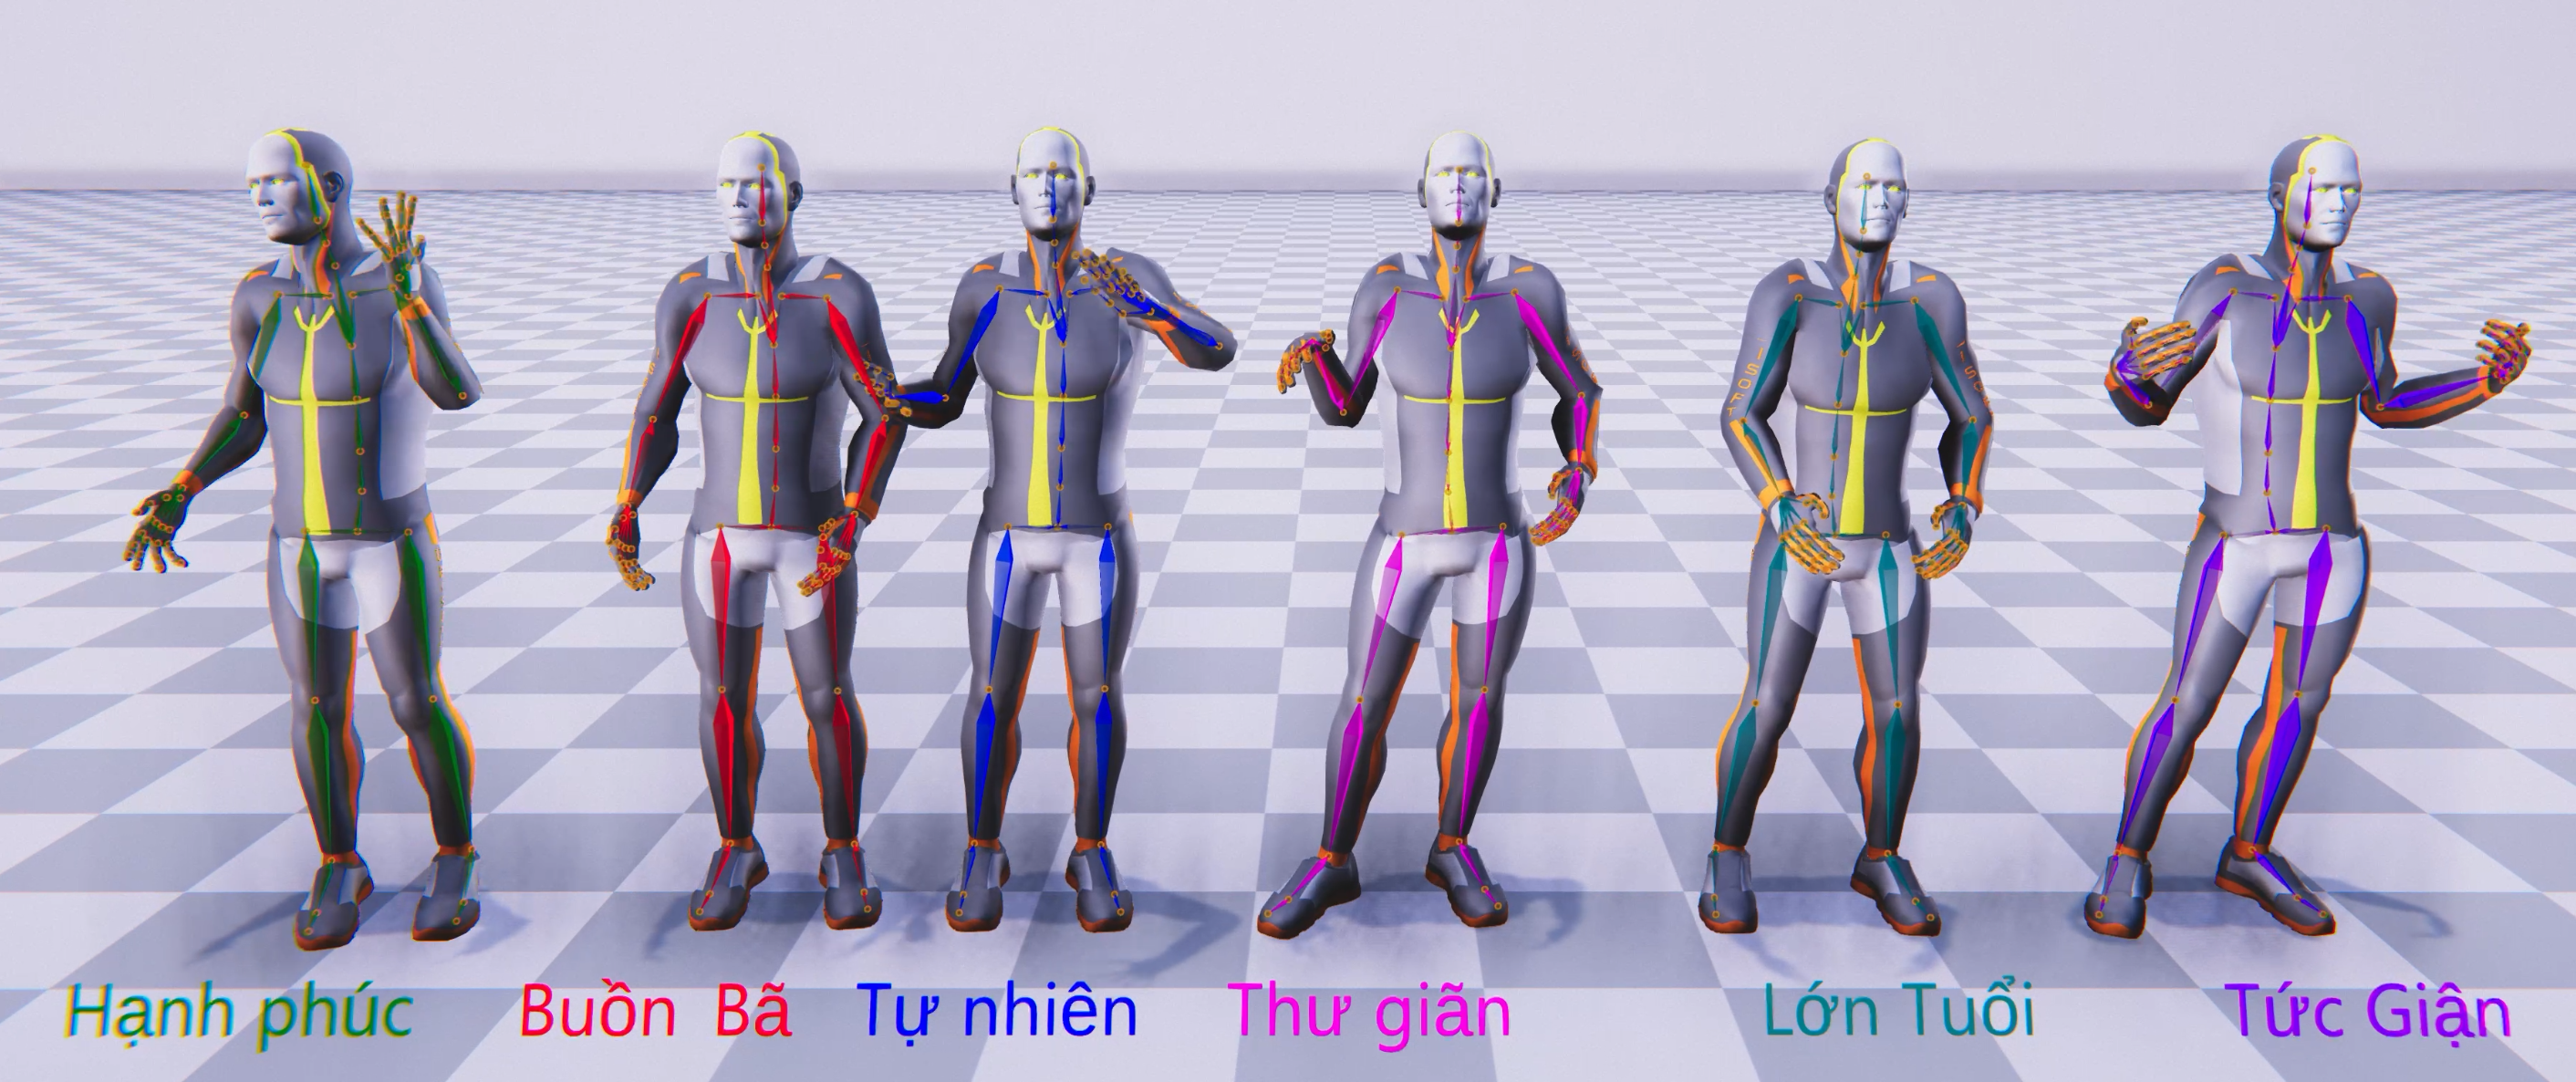
\includegraphics[width=\textwidth]{figures/ListOfEmotion}
  \caption{Gesture generation result in various emotion, speech and text}
  \label{fig:teaser}
\end{teaserfigure}

%%
%% This command processes the author and affiliation and title
%% information and builds the first part of the formatted document.
\maketitle

%%
%% Sections.
\section{Introduction}
\label{sec:introduction}

Every day, billions of people around the world look at RGB screens, and the output displayed on these screens is the result of various software systems. Therefore, the rendering of each pixel on the screen and the realistic simulation of images have been a focus of computer graphics scientists since the 1960s, particularly in the simulation of human figures or digital human.

Today, computer graphics technology can realistically simulate many complex objects such as water, roads, bread, and even human bodies and faces with incredible detail, down to individual hair strands, pimples, and eye textures. In 2015, using 3D scanning techniques \cite{metallo2015scanning} to capture all angles of the face and light reflection, researchers were able to recreate President Obama's face on a computer with high precision, making it almost indistinguishable from the real thing.

Artificial intelligence (AI) has shown remarkable results in recent years, not only in research but also in practical applications, such as ChatGPT and Midjourney, showcasing vertical and horizontal growth in various fields. Although computer graphics can construct highly realistic human faces, gesture generation has traditionally relied on Motion Capture from sensors, posing significant challenges in building an AI system that learns from data. Generating realistic beat gestures is challenging because gestural beats and verbal stresses are not strictly synchronized, and it's complicating for end-to-end learning models to capture the complex relationship between speech and gestures.



Modern AI systems can now generate human-like text and speech. However, one of the biggest obstacles in building digital humans is gesture generation. Therefore, the aim of this paper is to build an emotional and semantic-conditioned conversational gesture generation system using both text and speech as input.



\subsection{Problem Data}
\label{sec:Data}

%\begin{figure}[h]
%	\centering
%	\begin{subfigure}{0.48\linewidth}
%		\centering
%		\includegraphics[height=10cm]{images/Skeleton.png}
%		\caption{\small Skeleton and joint names of a frame}
%		\label{fig:Skeleton}
%	\end{subfigure}
%	\hfill
%	\begin{subfigure}{0.48\linewidth}
%		\centering
%		\includegraphics[height=10cm]{images/MotionPastAndFuture.png}
%		\caption{\small Motion sequence consisting of 6 past and 6 future gestures}
%		\label{fig:MotionPastAndFuture}
%	\end{subfigure}
%\end{figure}

\begin{figure}[h]
	\centering
	\centering
	\includegraphics[height=10cm]{images/Skeleton.png}
	\caption{\small Skeleton and joint names of a frame}
	\label{fig:Skeleton}
\end{figure}

\subsubsection{Skeleton Structure of Gestures}

In this thesis, a gesture is defined as the movement of a character's entire body over time, as shown in \autoref{fig:Skeleton}, captured frame by frame. In computer graphics, character motion is represented as bone-specific movements, including hands, legs, head, spine, etc. The full character skeleton structure is presented in Appendix \autoref{appendix:BVHData:skeleton}.

Motion data is captured via motion capture systems using cameras and specialized sensors. The output is typically stored in BVH (Biovision Hierarchy) files.

A BVH file consists of two main parts: `HIERARCHY` and `MOTION`. The `HIERARCHY` section is structured as a tree containing the skeleton’s initial positions and names. The `MOTION` section contains the movement data for the entire skeleton frame-by-frame. Each BVH file includes frame rate (fps) and total frame count. Details are presented in Appendix \autoref{appendix:BVHData:BVHStructure}.

\subsubsection{Motion Structure of Gestures}

Gesture motion data, as illustrated in \autoref{fig:MotionPastAndFuture}, or the `MOTION` section of a BVH file, contains position and rotation information per frame. Each frame is a skeleton of 75 bones: $\{ \textbf{b}_{1}, \textbf{b}_{2}, \cdots , \textbf{b}_{75} \}$, where each bone has position $\{ p_{x}, p_{y}, p_{z} \}$ and rotation $\{ r_{x}, r_{y}, r_{z} \}$.

The output of gesture generation is a sequence of bone rotations per frame. The generated gestures are evaluated based on naturalness, human-likeness, and contextual appropriateness.

In this thesis, the skeleton’s position and rotation data are preprocessed into a feature vector $\mathbf{g} \in \mathbb{R}^{D}$ with $D = 1141$. The learning data becomes $\bx \in \mathbb{R}^{M \times D}$. The preprocessing pipeline is detailed in \autoref{appendix:BVHData}.

\subsection{Problem Statement}
\label{sec:ProblemStatement}

The ultimate goal is to produce a sequence of gestures that reflect the motion of the skeleton frame by frame. This can be approached via classification, clustering, or regression. In this thesis, gesture generation is framed as a regression problem: given an input gesture sequence, predict the next sequence.

\begin{figure}[h]
	\centering
	\href{https://www.youtube.com/watch?v=B6nv1kQmi-Q}{\includegraphics[width=\linewidth]{images/FeatureProcessing}}
	\caption{A gesture sequence: the first $N$ frames are used as seed gesture $\mathbf{s}$, and the remaining $M$ frames are to be predicted}
	\label{fig:GestureSeries}
\end{figure}

Each gesture sequence is labeled with an emotion. A key novelty of this thesis is pairing the gesture sequence with both the original speech and the corresponding text (transcribed from the speech).

The objective is to build a model that predicts $M$ future frames from the given inputs: seed gesture $\mathbf{s} \in \mathbb{R}^{1:N \times D}$, speech $\mathbf{a}$, text $\mathbf{v}$, and emotion $\mathbf{e}$.

The model prediction is $\hat{\mathbf{x}} \in \mathbb{R}^{1:M \times D}$, which is compared against ground-truth gesture $\mathbf{x} \in \mathbb{R}^{1:M \times D}$.

\begin{multicols}{2}
	
	\textbf{Input}
	
	\begin{itemize}
		\item Seed gesture sequence: $\mathbf{s} \in \mathbb{R}^{1:N \times D}$
		\item Speech signal: $\mathbf{a}$
		\item Text: $\mathbf{v}$
		\item Emotion: $\mathbf{e}$ 
		
		{\small
			(\texttt{Happy},  \texttt{Sad},  \texttt{Neutral}, \texttt{Angry}, \texttt{Old}, \texttt{Funny})
		}
	\end{itemize}
	
	\columnbreak
	
	\textbf{Predicted Output}
	\begin{itemize}
		\item Predicted gesture sequence:
		$\hat{\mathbf{x}} \in \mathbb{R}^{1:M \times D}$
	\end{itemize}
	
	\textbf{Ground Truth}
	\begin{itemize}
		\item Ground truth gesture: $ \mathbf{x}  \in \mathbb{R}^{1:M \times D}$
	\end{itemize}
	
\end{multicols}

\subsection{Challenges}
\label{sec:difficult}

There are several challenges in building a model that can learn human-like conversational gesture patterns:

1. \textit{Limited and low-quality data:} Creating large-scale, high-quality datasets for motion capture is extremely costly in the industry.

2. \textit{Inconsistent context between modalities:} Text datasets are more abundant than speech, and speaker attribution is often missing. Synchronization between speech and emotional tone is also lacking. Additionally, training texts span many unrelated topics.

3. \textit{Imbalanced feature distributions:} Current datasets are biased toward English-speaking gestures, with imbalanced gesture distributions between speaking, questioning, and silent states.

4. \textit{High computational cost due to multimodal input:} The model must encode text, speech, and 3D pose data, increasing the computational load during both training and inference. Reducing input information also degrades performance.

5. \textit{Sequential preprocessing steps:} Although human-computer interaction is most effective through speech and keyboard input, processing the text and speech input for gesture generation must be done sequentially. In real-world applications, inference latency is critical, and users cannot wait long. Rendering the gestures on screen must also be optimized for speed.

\subsection{Contributions}

 In summary, our main contributions in this paper are:
 
\begin{itemize}
	\item From existing datasets, speech is transcribed into text and used as additional semantic features for training.
	
	\item Based on the DiffuseStyleGesture model, the thesis extends the conditional denoising process to include text features.
	
	\item The thesis uses Unity for rendering, data extraction, and visualization of gesture generation results.
	
	\item The thesis develops a rendering pipeline and demonstrates the system with Unity.
\end{itemize}



%The main contributions of our work are as follows: 
% In summary, our main contributions in this paper are:
% \begin{itemize}
%     \item We present a novel rhythm- and semantics-aware co-speech gesture synthesis system that generates natural-looking gestures. To the best of our knowledge, this is the first neural system that explicitly models both the rhythmic and semantic relations between speech and gestures.
%     \item We develop a robust rhythm-based segmentation pipeline to ensure the temporal coherence between speech and gestures, which we find is crucial to achieving rhythmic gestures.
%     \item We devise an effective mechanism to relate the disentangled multi-level features of both speech and motion, which enables generating gestures with convincing semantics.
% \end{itemize}


%\section{INTRODUCTION}
%
%ICLR requires electronic submissions, processed by
%\url{https://openreview.net/}. See ICLR's website for more instructions.
%
%If your paper is ultimately accepted, the statement {\tt
	%  {\textbackslash}iclrfinalcopy} should be inserted to adjust the
%format to the camera ready requirements.
%
%The format for the submissions is a variant of the NeurIPS format.
%Please read carefully the instructions below, and follow them
%faithfully.
%
%\subsection{Style}
%
%Papers to be submitted to ICLR 2025 must be prepared according to the
%instructions presented here.
%
%%% Please note that we have introduced automatic line number generation
%%% into the style file for \LaTeXe. This is to help reviewers
%%% refer to specific lines of the paper when they make their comments. Please do
%%% NOT refer to these line numbers in your paper as they will be removed from the
%%% style file for the final version of accepted papers.
%
%Authors are required to use the ICLR \LaTeX{} style files obtainable at the
%ICLR website. Please make sure you use the current files and
%not previous versions. Tweaking the style files may be grounds for rejection.
%
%\subsection{Retrieval of style files}
%
%The style files for ICLR and other conference information are available online at:
%\begin{center}
%   \url{http://www.iclr.cc/}
%\end{center}
%The file \verb+iclr2025_conference.pdf+ contains these
%instructions and illustrates the
%various formatting requirements your ICLR paper must satisfy.
%Submissions must be made using \LaTeX{} and the style files
%\verb+iclr2025_conference.sty+ and \verb+iclr2025_conference.bst+ (to be used with \LaTeX{}2e). The file
%\verb+iclr2025_conference.tex+ may be used as a ``shell'' for writing your paper. All you
%have to do is replace the author, title, abstract, and text of the paper with
%your own.
%
%The formatting instructions contained in these style files are summarized in
%sections \ref{gen_inst}, \ref{headings}, and \ref{others} below.



%\section{General formatting instructions}
%\label{gen_inst}
%
%The text must be confined within a rectangle 5.5~inches (33~picas) wide and
%9~inches (54~picas) long. The left margin is 1.5~inch (9~picas).
%Use 10~point type with a vertical spacing of 11~points. Times New Roman is the
%preferred typeface throughout. Paragraphs are separated by 1/2~line space,
%with no indentation.
%
%Paper title is 17~point, in small caps and left-aligned.
%All pages should start at 1~inch (6~picas) from the top of the page.
%
%Authors' names are
%set in boldface, and each name is placed above its corresponding
%address. The lead author's name is to be listed first, and
%the co-authors' names are set to follow. Authors sharing the
%same address can be on the same line.
%
%Please pay special attention to the instructions in section \ref{others}
%regarding figures, tables, acknowledgments, and references.
%
%
%There will be a strict upper limit of 10 pages for the main text of the initial submission, with unlimited additional pages for citations. 

\section{RELATED WORK}
\label{sec:related_work}


Gesture generation, like other machine learning tasks, has been explored using both traditional rule-based methods and modern data-driven approaches. We first examine the fundamental characteristics of gestures (\autoref{sec:relationspeechandgesture}) as a basis for modeling their relationship with text and speech. \autoref{fig:CommonStage} illustrates the common processing stages shared across various gesture generation techniques.


\subsection{Gesture Characteristics}
\label{sec:relationspeechandgesture}

According to linguistics, gestures can be categorized into six main groups: adaptors, emblems, deictics, iconics, metaphorics, and beats \citep{ekman1969repertoire}, \citep{sebeok2011advances}. Among them, beat gestures do not carry direct semantic meaning but play an important role in synchronizing rhythm between speech and gesture \citep{kipp2005gesture}, \citep{sebeok2011advances}. However, the rhythm between speech and beat gestures is not fully synchronized, making the temporal alignment between them complex to model \citep{mcclave1994gestural}, \citep{bhattacharya2021speech2affectivegestures}, \citep{kucherenko2020gesticulator}, \citep{yoon2020speech}.

Gestures interact with various levels of information in speech \citep{sebeok2011advances}. For instance, emblematic gestures like a thumbs-up are usually linked to high-level semantic content (e.g., “good” or “excellent”), while beat gestures often accompany low-level prosodic features such as emphasis. Previous studies typically extract features from the final layer of the speech encoder to synthesize gestures \citep{alexanderson2020style}, \citep{bhattacharya2021speech2affectivegestures}, \citep{kucherenko2021large}, \citep{qian2021speech}, \citep{yoon2022genea}. However, this approach may blend information from different levels, making it hard to disentangle rhythm and semantics.

As shown in linguistic studies \citep{kipp2005gesture}, \citep{neff2008gesture}, \citep{webb1997linguistic}, gestures in daily communication can be decomposed into a limited number of semantic units with various motion variations. Based on this assumption, speech features are divided into two types: high-level features representing semantic units and low-level features capturing motion variations. Their relationships are learned across different layers of the speech encoder. Experiments demonstrate that this mechanism can effectively disentangle features at different levels and generate gestures that are both semantically and stylistically appropriate.





\subsection{Overview of Gesture Generation Methods}
\label{sec:relatedwork}
%
%\subsubsection{Rule-Based Methods}
%
%These methods rely on clearly defined rules, which are manually crafted to determine how the system processes inputs to produce outputs.
%
%\textbf{Methods}: Representative rule-based methods include the \textit{Robot behavior toolkit} \citep{huang2012robot} and \textit{Animated conversation} \citep{cassell1994animated}. These approaches typically map speech to gesture units using handcrafted rules. Rule-based systems allow for straightforward control over model outputs and provide good interpretability.  
%However, the cost of manually designing these rules is prohibitive for complex applications requiring the processing of large-scale data.
%
%\subsubsection{Statistical Methods}
%
%These methods rely on data analysis, learning patterns from datasets, and using probabilistic models or mathematical functions for prediction. The approach involves optimizing model parameters to fit the data.
%
%
%\textbf{Methods}: Like rule-based methods, data-driven methods also map speech features to corresponding gestures. However, instead of manual rules, they employ automatic learning based on statistical data analysis.
%
%Representative statistical approaches include \textit{Gesture controllers} \citep{levine2010gesture}, \textit{Statistics-based} \citep{yang2020statistics}, which use probabilistic distributions to find similarities between speech and gesture features. \textit{Gesture modeling} \citep{neff2008gesture} constructs probabilistic models to learn individual speaker styles.
%
%\subsubsection{Deep Learning Methods}
%
%These methods utilize multi-layer perceptrons (MLPs) to automatically extract features from raw data and learn complex data representations through parameter optimization.
%
%%\begin{figure}[b]
%%	\centering
%%	\includegraphics[width=\linewidth]{figures/GeneralOverview}
%%	\caption{Overview of different generative models.}
%%	\label{fig:GeneralOverview}
%%\end{figure}
%
%Deep learning-based gesture generation methods can be divided into two main groups: likelihood-based models and implicit generative models \citep{song2021score}.
%
%
%\textbf{Likelihood-Based Models}
%
%These models work by maximizing the likelihood of observed data given model parameters $\theta$. The objective is to find the optimal parameters $\theta'$ by modeling the probability $p(\mathbf{x})$ of the data, where $\mathbf{x}$ represents the gesture sequence.
%
%
%\textbf{Methods}: The application of deep learning to gesture generation has evolved alongside the development of deep learning models, including RNNs, LSTMs, and Transformers. Representative likelihood-based methods include:
%
%\begin{itemize}
%	\item \textit{Gesticulator} \citep{kucherenko2020gesticulator}, which uses a Multilayer Perceptron (MLP) to encode text and audio features, with BERT-derived vectors used as text features.
%	
%	\item \textit{HA2G} \citep{liu2022learning} builds a hierarchical Transformer-based model to learn multi-level correlations between speech and gestures, from local to global features.
%	
%	\item \textit{Gesture Generation from Trimodal Context} \citep{yoon2020speech} uses an RNN architecture and treats gesture generation as a translation task in natural language processing.
%	
%	\item \textit{DNN} \citep{chiu2015predicting} combines LSTM and GRU to build a classifier neural network that selects appropriate gesture units based on speech input.
%	
%	\item \textit{Cascaded Motion Network (CaMN)} \citep{liu2022beat} introduces the BEAT dataset and a waterfall-like model. Speaker information, emotion labels, text, speech, and gesture features are processed through layers to extract latent vectors. In the fusion stage, CaMN combines features sequentially: speaker and emotion features are merged first, followed by integration with latent vectors of text, speech, and gestures.
%	
%	\item \textbf{Motion Graph}: In \textit{Gesturemaster} \citep{zhou2022gesturemaster}, a semantic graph is constructed where words in a sentence are connected based on semantic relationships. The model then selects the most relevant nodes and edges in the graph to represent gestures.
%\end{itemize}


\textbf{Rule-Based Methods}
Robot Behavior Toolkit \citep{huang2012robot} and Animated Conversation \citep{cassell1994animated} use manually crafted rules to map speech to gesture units. \textbf{Statistical Methods}
Gesture Controllers \citep{levine2010gesture} and Statistics-Based \citep{yang2020statistics} employ probabilistic distributions to align speech and gesture features, while Gesture Modeling \citep{neff2008gesture} captures individual speaker styles through probabilistic models, automating the mapping process compared to rule-based methods.
% These approaches offer clear control and interpretability but are labor-intensive for complex, large-scale applications.

\textbf{Deep Learning Methods}
Deep learning methods leverage multi-layer perceptrons to extract complex features from raw data. They are categorized into likelihood-based and implicit generative models \citep{song2021score}.

\textit{Likelihood-Based Models}

These models optimize the likelihood of gesture sequences given model parameters. Key methods include:
\begin{itemize}
	\item \textit{Gesticulator} \citep{kucherenko2020gesticulator}: Uses MLPs to encode text and audio, with BERT-derived text features.
	\item \textit{HA2G} \citep{liu2022learning}: Employs a hierarchical Transformer to model speech-gesture correlations.
	\item \textit{Gesture Generation from Trimodal Context} \citep{yoon2020speech}: Treats gesture generation as a translation task using RNNs.
	\item \textit{DNN} \citep{chiu2015predicting}: Combines LSTM and GRU for gesture classification based on speech.
	\item \textit{CaMN} \citep{liu2022beat}: Processes speaker, emotion, text, speech, and gesture features in a cascaded network, fusing them sequentially.
	\item \textit{Gesturemaster} \citep{zhou2022gesturemaster}: Constructs a semantic graph to select gesture-representing nodes and edges.
\end{itemize}

%\vfill
%\begin{figure*}[htbp]
%	\centering
%	\includegraphics[width=0.9\linewidth]{figures/CommonStage.png}
%	\caption{Common stages in gesture generation models.}
%	\label{fig:CommonStage}
%\end{figure*}

\begin{figure*}[htbp]
	\centering
	\includegraphics[width=0.9\linewidth]{figures/CommonStage.png}
%	\resizebox{\textwidth}{!}{%\begin{tikzpicture}[
%	box/.style={rounded corners, draw, fill=#1, minimum width=2cm, minimum height=1cm, align=center},
%	arrow/.style={->, >=stealth},
%	cylinder/.style={shape=cylinder, draw, minimum height=1.5cm, minimum width=0.8cm, shape aspect=2, align=center}
%	]
%	
%	% Boxes
%	\node[box=#e1d5e7, fill=#e1d5e7, draw=#9673a6] (preprocess) at (2,-3) {\textbf{1. Pre-processing}};
%	\node[box=#ffe6cc, fill=#ffe6cc, draw=#d79b00, right=1cm of preprocess] (featureproc) {2. Feature Processing};
%	\node[box=#dae8fc, fill=#dae8fc, draw=#6c8ebf, right=1cm of featureproc] (featureext) {\textbf{3. Feature Extraction}};
%	\node[box=#d5e8d4, fill=#d5e8d4, draw=#82b366, right=1cm of featureext] (featureenc) {\textbf{4. Feature Encoding}};
%	\node[box=#f8cecc, fill=#f8cecc, draw=#b85450, right=1cm of featureenc] (featurefus) {5. Feature Fusion};
%	\node[box=#d5e8d4, fill=#d5e8d4, draw=#82b366, right=1cm of featurefus] (featuredec) {\textbf{6. Feature Decoding}};
%	\node[box=#fff2cc, fill=#fff2cc, draw=#d6b656, right=1cm of featuredec] (render) {\textbf{7. Render}};
%	
%	% Cylinder
%	\node[cylinder, below left=0.5cm and 1cm of preprocess] (motiondata) {Motion\\Data};
%	
%	% Model box
%	\node[rounded corners, draw, fill=#f5f5f5, minimum width=6cm, minimum height=0.7cm, above=0.5cm of featureext] (model) {$\text{Model}_\theta$};
%	
%	% Arrows
%	\draw[arrow] (motiondata.east) -- (preprocess.west);
%	\draw[arrow] (preprocess) -- (featureproc);
%	\draw[arrow] (featureproc) -- (featureext);
%	\draw[arrow] (featureext) -- (featureenc);
%	\draw[arrow] (featureenc) -- (featurefus);
%	\draw[arrow] (featurefus) -- (featuredec);
%	\draw[arrow] (featuredec) -- (render);
%	
%\end{tikzpicture}

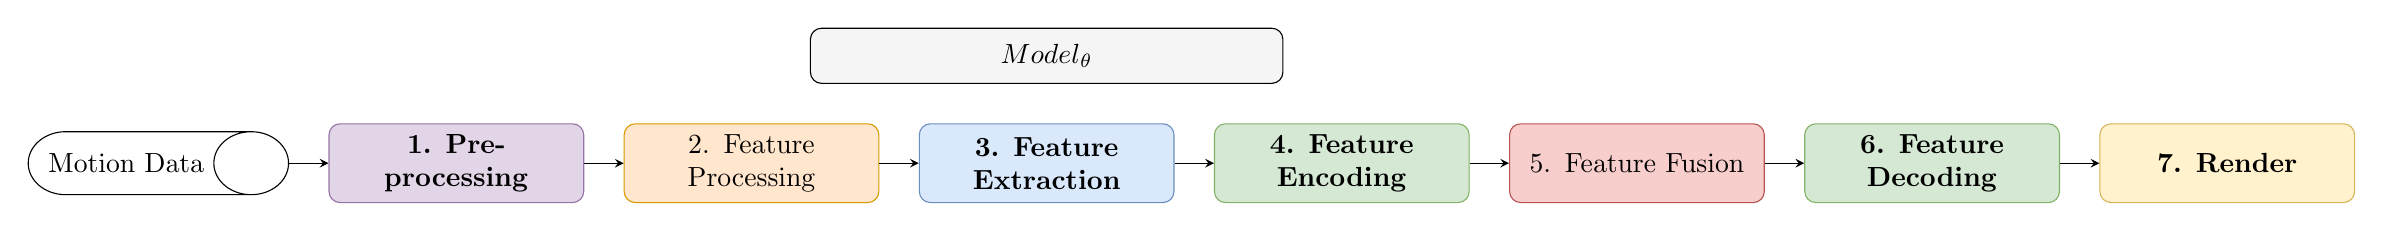
\begin{tikzpicture}[
	box/.style={rounded corners, draw, fill=#1, minimum width=2cm, minimum height=1cm, text width = 30mm,align=center},
	arrow/.style={->, >=stealth},
	cylinder/.style={shape=cylinder, draw, minimum height=1.5cm, minimum width=0.8cm, shape aspect=2, align=center}
	]
	
	% Boxes
	\node[draw=preprocessdraw, fill=preprocessfill, box=preprocessfill] (preprocess) at (2,-3) {\textbf{1. Pre-processing}};
	\node[draw=featureprocdraw, fill=featureprocfill, box=featureprocfill, right=0.5cm of preprocess] (featureproc) {2. Feature Processing};
	\node[draw=featureextdraw, fill=featureextfill, box=featureextfill, right=0.5cm of featureproc] (featureext) {\textbf{3. Feature Extraction}};
	\node[draw=featureencdraw, fill=featureencfill, box=featureencfill, right=0.5cm of featureext] (featureenc) {\textbf{4. Feature Encoding}};
	\node[draw=featurefusdraw, fill=featurefusfill, box=featurefusfill, right=0.5cm of featureenc] (featurefus) {5. Feature Fusion};
	\node[draw=featuredecdraw, fill=featuredecfill, box=featuredecfill, right=0.5cm of featurefus] (featuredec) {\textbf{6. Feature Decoding}};
	\node[draw=renderdraw, fill=renderfill, box=renderfill, right=0.5cm of featuredec] (render) {\textbf{7. Render}};
	
	% Cylinder
	\node[cylinder, left=0.5cm and 0.5cm of preprocess] (motiondata) {\text{Motion Data}};
	
	% Model box
	\node[rounded corners, draw, fill=modelfill, minimum width=6cm, minimum height=0.7cm, above=0.5cm of featureext] (model) {$\text{Model}_\theta$};
	
	% Arrows
	\draw[arrow] (motiondata.east) -- (preprocess.west);
	\draw[arrow] (preprocess) -- (featureproc);
	\draw[arrow] (featureproc) -- (featureext);
	\draw[arrow] (featureext) -- (featureenc);
	\draw[arrow] (featureenc) -- (featurefus);
	\draw[arrow] (featurefus) -- (featuredec);
	\draw[arrow] (featuredec) -- (render);
	
\end{tikzpicture}}
	\caption{Common stages in gesture generation models.}
	\label{fig:CommonStage}
\end{figure*}

\textbf{Implicit Generative Models}
\label{sec:ImplicitGenerativeModels}

Implicit generative models learn the data distribution without explicitly modeling the probability density function $p(\bx)$. Instead of directly computing $p(\bx)$, the model learns a mapping $G_{\theta}: \mathcal{Z} \to \mathcal{X}$ by matching the distributions between real and generated data $\mathbf{x} = G_\theta(\mathbf{z}), \quad \mathbf{z} \sim p_z(\mathbf{z})$. Here, $\mathcal{Z}$ denotes the input noise space, typically with a simple distribution \(p_{z}\) (e.g., Gaussian, Uniform), and \(\mathcal{X}\) is the space of real data, which in this case is gesture sequences \(\mathbf{x}\).

In gesture generation, to incorporate conditions such as speech or text labels, implicit generative models often introduce a condition $\mathbf{c}$ representing the context of the task, resulting in the conditional generation: $\mathbf{x} = G_\theta(\mathbf{z}, \mathbf{c})$. This context may include speech, text, speaker ID, style, emotion, or initial gestures.

A typical example is the generative adversarial network (GAN) and Diffusion model, where data is synthesized by transforming an initial simple distribution (e.g., Gaussian) into the target data distribution.


\textbf{Methods}: Representative implicit generative models include:

\begin{itemize}
	\item \textit{MoGlow} \citep{henter2020moglow} uses Normalizing Flows to maintain motion consistency and compatibility, while providing control via input parameters. This allows users to generate new motions or modify existing ones by adjusting control parameters.
	
	\item \textbf{GAN}: \textit{GRU-based WGAN} \citep{wu2021probabilistic} utilizes Wasserstein GAN to evaluate and improve the quality of gesture synthesis. The model focuses on optimizing the Wasserstein loss, mitigating mode collapse typically seen in traditional GANs. GRUs process speech data and convert it into usable gesture features, which are then fed into the WGAN for evaluation and refinement.
	
	\item \textbf{VAE}: \textit{FreeMo} \citep{xu2022freeform} employs a VAE to decompose gestures into pose modes and rhythmic motions. Gesture poses are randomly sampled using conditional sampling in the VAE's latent space, while rhythmic motions are generated from...
	
	\item \textbf{VQ-VAE}: \textit{Rhythmic Gesticulator} \citep{ao2022rhythmic} preprocesses speech segments based on beats, dividing speech into smaller parts and representing them as blocks with normalized dimensions. Similar to the VQ-VAE approach, normalized gesture sequences are quantized into discrete gesture lexicons. The model learns the gesture vocabulary conditioned on the previous gesture, gesture style, and speech. It then reconstructs the gesture sequence via denormalization. Unlike generative models like GANs or Diffusion, VQ-VAE focuses more on compression rather than direct generation.
	
	\item \textbf{Diffusion}: Diffusion models focus on generating new data from noisy inputs by progressively denoising toward the original data. Diffusion-based approaches will be presented in \autoref{sec:diffusionbase}.
\end{itemize}



%
%\subsection{Common Stages in Deep Learning Approaches for Gesture Generation}
%\label{sec:commonstage}
%
%As presented in \autoref{sec:Data}, gestures consist of sequences of 3D point coordinates. For each dataset, the number of bones per frame may vary.
%
%
%Deep learning approaches to gesture generation are implemented using various techniques. However, we generalize the process into the following main stages, illustrated in \autoref{fig:CommonStage}:
%
%
%\begin{enumerate}
%	\item \textbf{Preprocessing}: In the preprocessing stage, data such as speech segments, gesture sequences, and text are read and digitized into vectors or matrices that represent raw data information. Depending on the specific learning method, the selected initial data features may vary.
%	
%	\item \textbf{Feature Processing}: In this stage, raw data such as speech and text are embedded into feature vectors. Different methods use different embedding models. The way gesture sequences are represented as feature vectors also varies across methods.
%	
%	\item \textbf{Feature Extraction}: This stage uses linear transformation layers or CNN layers to extract features from the data. Text and speech features, after being processed, may be further passed through feature extraction layers to generate representation vectors corresponding to the input modalities.
%	
%	\item \textbf{Feature Encoding}: In this stage, gesture, emotion, and speech vectors are encoded into a lower-dimensional latent space to facilitate learning the correlations among modalities in the feature fusion stage.
%	
%	\item \textbf{Feature Fusion}: In this stage, features from speech, text, gestures, and other information are combined, typically using concatenation, fully connected layers, or operations such as vector addition or subtraction in the latent space.
%	
%	\item \textbf{Feature Decoding}: In this stage, latent vectors are decoded or upsampled back to their original dimensionality.
%	
%	\item \textbf{Rendering}: Once the output vectors are restored to their original size, they are converted back into BVH files and rendered using software such as Blender or Unity to visualize character motion.
%\end{enumerate}





\subsection{Diffusion-based Model for Gesture Generation}
\label{sec:diffusionbase}




\begin{itemize}
	\item \textit{MotionDiffuse} \citep{zhang2022motiondiffuse} employs a conditional Diffusion model, with conditions based solely on text, excluding audio. Additionally, the model predicts noise rather than directly predicting the original gesture sequence. MotionDiffuse utilizes Self-Attention and Cross-Attention layers to model the correlation between textual features and gesture features during \textit{Stage 5. Feature Fusion} (\autoref{fig:CommonStage}).
	
	\item \textit{Flame} \citep{kim2023flame} applies a Diffusion model with a Transformer-based architecture. In \textit{Stage 2. Feature Processing} (\autoref{fig:CommonStage}), it uses the pre-trained RoBERTa model to embed the text into textual feature vectors, which serve as the conditioning input. During \textit{Stage 5. Feature Fusion} (\autoref{fig:CommonStage}), the text is used as the $\texttt{CLS}$ token prepended to the gesture sequence before passing through the Transformer Decoder. Similar to other methods, the model predicts the added noise rather than the original gesture sequence.
	
	\item \textit{DiffWave} \citep{kong2020diffwave} is a noise-predicting Diffusion model in which the time steps pass through multiple Fully Connected layers and a Swish activation function before feature fusion. It uses a dilated convolutional architecture inherited from WaveNet. DiffWave enables better representation of speech, improving the effectiveness of conditioning for the Diffusion model.
	
	\item \textit{Listen, Denoise, Action} \citep{alexanderson2022listen} builds upon DiffWave \citep{kong2020diffwave}, replacing the dilated convolution layers with a Transformer, and integrating Conformer modules to enhance model performance.
	
	\item \textit{DiffSHEG} \citep{chen2024diffsheg} employs a Diffusion model; in \textit{Stage 2. Feature Processing}, it uses HuBERT to encode the audio signal. The model treats facial expressions as a signal for gesture generation and achieves real-time fusion of both facial expressions and gestures.
	
	\item \textit{GestureDiffuCLIP} \citep{ao2023gesturediffuclip} uses a Diffusion model conditioned on text, leveraging Contrastive Learning with CLIP to integrate text features and control gesture styles. Similar to other prompt-based approaches such as StableDiffusion or Midjourney, it treats text as prompts to learn gestures from descriptive sentences.
	
	\item \textit{Freetalker} \citep{yang2024freetalker} trains a Diffusion model on multiple datasets to generate speaker-specific gestures conditioned on speech and text. Unlike Transformer-based methods, Freetalker employs an Attention-based Network to model the correlation between textual, auditory, and gesture features during \textit{Stage 5. Feature Fusion} (\autoref{fig:CommonStage}).
\end{itemize}

%\begin{figure}[htbp]
%	\centering
%	\includegraphics[width=\linewidth]{figures/ScoreMatching.jpg}
%	\caption{Illustration of the diffusion drift term in gesture generation. The figure demonstrates how the learned drift guides the reverse diffusion process to synthesize temporally coherent and semantically relevant gestures from noise.}
%	\label{fig:ScoreMatching}
%\end{figure}

\vspace{-0.2cm}
\subsubsection{Selected Diffusion-based Methods}


\begin{itemize}
	\item \textit{MDM} \citep{tevet2022human} applies conditional Diffusion to gesture generation, using CLIP (Contrastive Language–Image Pre-training) embeddings of descriptive text as conditions. MDM adopts a Transformer-based architecture to reconstruct original gesture data. Like other text-based Diffusion approaches, in \textit{Stage 3. Feature Extraction} (\autoref{fig:CommonStage}), the input text is randomly masked to hide certain segments, enabling the model to learn the importance of each part for various gestures. 
	
	In \textit{Stage 5. Feature Fusion} (\autoref{fig:CommonStage}), the text is prepended as a $\texttt{[CLS]}$ token to the gesture sequence before passing through the Transformer Encoder, where self-attention models the relationship between the text and each gesture frame. MDM predicts the original gesture data rather than noise.
	
	\item \textbf{DiffuseStyleGesture} \citep{yang2023diffusestylegesture} extends \textit{MDM} \citep{tevet2022human} by incorporating audio, initial gestures, and style as conditioning inputs. In \textit{Stage 1. Preprocessing} (\autoref{fig:CommonStage}), the model processes coordinate vectors to obtain feature vectors of dimension $D=1141$ per frame. In \textit{Stage 2. Feature Processing} (\autoref{fig:CommonStage}), DiffuseStyleGesture uses WavLM for audio embedding. In \textit{Stage 5. Feature Fusion} (\autoref{fig:CommonStage}), it improves upon MDM by applying Cross-Local Attention prior to the Transformer Encoder.
\end{itemize}
%
%\subsubsection{Comparison of Gesture Generation Methods}
%
%
%\begin{table*}[t]
%	\small
%	\centering
%	\renewcommand{\arraystretch}{1.5}
%	\resizebox{\textwidth}{!}{
%		\begin{tabular}{|p{0.2\textwidth}|p{0.35\textwidth}|p{0.35\textwidth}|p{0.2\textwidth}|}
%			\hline
%			\textbf{Representative Method} & \textbf{Advantages} & \textbf{Disadvantages} & \textbf{Method Type} \\ \hline
%			Robot behavior toolkit \citep{huang2012robot} & 
%			- Easy to understand and implement. \newline 
%			- Highly interpretable and controllable. \newline
%			- Effective for simple cases or small datasets. & 
%			- Does not generalize well to complex data. \newline 
%			- Labor-intensive rule construction. & 
%			Rule-based model \\ \hline
%			MLP \citep{kucherenko2020gesticulator}, RNN \citep{bhattacharya2021speech2affectivegestures}, \citep{liu2022learning}, \citep{hasegawa2018evaluation}, \citep{yoon2020speech}, CNN \citep{habibie2021learning}, Transformer \citep{bhattacharya2021text2gestures}  & 
%			- Able to estimate data probability density. \newline 
%			- Scalable and learns well from large datasets. & 
%			- Sensitive to noise. \newline 
%			- Performs poorly on low-frequency data. \newline
%			- Low diversity in generation. & 
%			Likelihood-based model \\ \hline
%			\textbf{DiffusionStyle-Gesture} \citep{yang2023diffusestylegesture}, MDM \citep{tevet2022human}, Motiondiffuse \citep{zhang2022motiondiffuse} &
%			- Generates high-quality data. \newline 
%			- Flexible and diverse outputs. \newline
%			- Covers low-density regions of data space. & 
%			- Requires complex configuration for optimal performance. \newline 
%			- Random noise leads to different outputs each time. \newline 
%			- Slow sampling process. & 
%			Implicit generative model \\ \hline
%		\end{tabular}
%	}
%	\caption{Comparison of advantages and disadvantages of different methods}
%	\label{table:CompareMethod}
%\end{table*}



\input{sections/3_system_overview}



\section{EXPERIMENTS AND RENDERING}
\label{sec:results}


\subsection{Dataset}

%\begin{figure}[H]
%	\centering
%	\includegraphics[width=\linewidth]{images/EmotionAnimation}
%	\caption{Illustration of 6 gestures: $\texttt{Happy}$, $\texttt{Sad}$, $\texttt{Neutral}$, $\texttt{Old}$, $\texttt{Relaxed}$, and $\texttt{Angry}$}
%\end{figure}

\begin{figure}[H]
	\centering
	\includegraphics[width=\linewidth]{images/DifferenceEmotion}
	\caption{Gesture sample of difference emotion}
	\Description{Gesture sample of difference emotion}
\end{figure}

This thesis uses the ZeroEGGS dataset \cite{ghorbani2022zeroeggszeroshotexamplebasedgesture}, a motion capture dataset designed for research and development of gesture generation models. It includes 67 monologue clips performed by a female motion capture actor, with a total duration of 135 minutes. The monologues are annotated with 6 different emotions: $\texttt{Happy}$, $\texttt{Sad}$, $\texttt{Neutral}$, $\texttt{Old}$, $\texttt{Relaxed}$, and $\texttt{Angry}$, enabling simulation of various emotional states in gestures and body movements. ZeroEGGS provides a rich platform for studying the integration of speech and dynamic gestures, supporting the development of models capable of adapting gestures according to emotions and text semantics.

\subsection{Data Preprocessing}
\label{sec:Preprocessing}

In stage {1. Data Preprocessing} (\autoref{fig:CommonStage}), gesture, speech, and text data are read and processed to be represented as vectors or matrices containing information derived from raw data.

For \textbf{text data}: the thesis uses the $\texttt{nltk}$ library for tokenization and $\texttt{contractions}$ to normalize contracted words.

One contribution of the thesis is to convert the speech data available in ZeroEGGS using Adobe Speech To Text, then align the phonetic timestamps using the Montreal Forced Aligner \cite{saxon2020robust} with an English phoneme dictionary to match the gesture frame rate, generating TextGrid files. From these TextGrids containing word-level timing information, the thesis uses $\texttt{gensim}$ to generate word2vec embeddings.

\textbf{Gesture data} consists of BVH (BioVision Motion Capture) files captured via motion capture systems. BVH files include two components: Hierarchy and Motion. Specifically:

\begin{itemize}
	\item \texttt{HIERARCHY}: defines a skeletal tree containing 75 bones $\{ \mathbf{b}_1, \mathbf{b}_2 \cdots \mathbf{b}_{75} \}$, each with an initial position (\texttt{OFFSET}) and \texttt{CHANNELS} parameters specifying the type and order of rotation angles (\texttt{Zrotation}, \texttt{Yrotation}, \texttt{Xrotation}) and position (\texttt{Xposition}, \texttt{Yposition}, \texttt{Zposition}), which are defined in the \texttt{MOTION} section. The first bone (usually \texttt{Hips}) is the root bone $\mathbf{b}_{\text{root}}$, used to define the T-pose via forward kinematics as the initial pose of the skeleton before applying motion.
	
	\item \texttt{MOTION}: a sequence of frames, each containing motion data representing changes of all $75$ bones as defined by the \texttt{CHANNELS} in the \texttt{HIERARCHY}.
\end{itemize}

The model in the thesis converts Euler rotation angles to quaternion rotation angles, where a quaternion is a 4-dimensional vector.

\begin{equation} \label{eq:gesturevector}
	\mathbf{g} = \Big[ \mathbf{p}_{\text{root}},  \mathbf{r}_{\text{root}},
	\mathbf{ p }'_{\text{root}},  \mathbf{r}'_{\text{root}},
	\mathbf{p}_{\text{joins}},  \mathbf{r}_{\text{joins}},
	\mathbf{p}'_{\text{joins}},  \mathbf{r}'_{\text{joins}},
	\mathbf{d}_{\text{gaze}}
	\Big]
\end{equation}

Here, each $\mathbf{g} \in \mathbb{R}^{1141}$ includes:
{
	\begin{itemize}
		\item $\mathbf{p}_{\text{root}} \in \mathbb{R}^3$: coordinates of the root joint
		\item $\mathbf{r}_{\text{root}} \in \mathbb{R}^4$: rotation (quaternion) of the root joint
		\item $\mathbf{p}'_{\text{root}} \in \mathbb{R}^3$: velocity of the root position
		\item $\mathbf{r}'_{\text{root}} \in \mathbb{R}^3$: angular velocity of the root rotation
		
		\item $\mathbf{p}_{\text{joins}} \in \mathbb{R}^{3 n_{\text{join} }}$: positions of other joints
		\item $\mathbf{r}_{\text{joins}} \in \mathbb{R}^{6 n_{\text{join} }}$: joint rotations on the X and Y planes
		\item $\mathbf{p}'_{\text{joins}} \in \mathbb{R}^{3n_{\text{join} }}$: velocity of joint positions
		\item $\mathbf{r}'_{\text{joins}} \in \mathbb{R}^{3n_{\text{join} }}$: angular velocity of joint rotations
		\item $\mathbf{d}_{\text{gaze}} \in \mathbb{R}^3$: gaze direction
\end{itemize}}

The original gesture sequences in Euler angles are converted to radians, then converted from Euler to Quaternion as detailed in \autoref{appendix:BVHData:QuaternionConvert}.

\textbf{Speech data}: $\mathbf{a}_{\text{raw}} \in \mathbb{R}^{ \text{length } }$ is raw speech sampled at 16000 Hz, trimmed into segments $\mathbf{a} \in \mathbb{R}^{64000}$ corresponding to 4 seconds. The thesis uses \texttt{ffmpeg-normalize} to normalize volume to a level lower than the original.

\textbf{Emotion}: Emotion data is represented using a predefined one-hot encoded vector. During sampling, the filename encodes the target emotion.

All data is stored using the $\texttt{h5}$ format.

\subsection{Training Process}

The entire model training process was conducted over approximately two weeks with the following parameters: number of training steps $T = 1000$, using an Nvidia 3090 GPU. The learning rate was set to $3 \times 10^{-5}$, batch size was $640$, and a total of $43,853$ samples were trained. At each step, $t$ is randomly sampled and input to $f_{\theta}$ to predict $\mathbf{x}_{0}$. The emotional control parameter was set to $\gamma = 0.1$. The probability of applying random masking to the emotion and initial gesture matrices was $10\%$, using a Bernoulli distribution to randomly hide/reveal these matrices.

The $\beta$ parameter was scheduled linearly from $0.5 \rightarrow 0.999$.

The $\operatorname{HuberLoss} (\mathbf{x}_{0},  \hat{\mathbf{x}}_{0} )$ is computed as follows:

\begin{itemize}
	\item If $|\mathbf{x}_0 - \hat{\mathbf{x}}_0| \leq \delta$ then $\mathcal{L}_{ \delta, \mathbf{x}_0, \hat{\mathbf{x}}_0} = \frac{1}{2} (\mathbf{x}_0 - \mathbf{x}_0)^2$: Below the threshold, the loss is computed as squared distance (similar to MSE), which is sensitive to small errors and provides smooth gradients.
	
	\item If $|\mathbf{x}_0 - \hat{\mathbf{x}}_0| > \delta$ then $\mathcal{L}_{ \delta, \mathbf{x}_0, \hat{\mathbf{x}}_0}  =  \delta \cdot |\mathbf{x}_0 - \mathbf{x}_0| - \frac{1}{2} \delta^2$: Above the threshold, the loss behaves like MAE, reducing sensitivity to large errors and improving robustness against outliers.
	
\end{itemize}

The training process is implemented in the open-source repository: \hyperlink{https://github.com/DeepGesture/DeepGesture}{Github/DeepGesture} \footnote{\url{https://github.com/DeepGesture/DeepGesture}}.

\subsection{Rendering Process in Unity}
\label{sec:Render}

To visualize the gesture generation process from model output, the thesis uses Unity in stage \textit{7. Rendering} (\autoref{fig:CommonStage}), extending code from the DeepPhase model \cite{starke2022deepphase}. The generated output is in BVH (BioVision Motion Capture) format. In Unity, the author adds C-Sharp scripts to render gestures based on coordinates and labels, with bone positions and rotations represented using quaternions.

Rendering details are presented in \autoref{Appendix3}.

The Unity project source code is available at: \hyperlink{https://github.com/DeepGesture/deepgesture-unity}{Github/DeepGesture-Unity}
\footnote{\url{https://github.com/DeepGesture/deepgesture-unity}}.










%\section{Data Preparation}
%\label{sec:data_preparation}
%The \emph{data} module of our system preprocesses an input speech, segments it into uniform blocks based on speech rhythms, and extracts features that will be used to generate co-speech gestures. In this section, we first introduce the representations of different speech modalities and gesture motion and then describe details of the data preprocessing.
%
%\subsection{Representation of Speech Modalities}
%
%\subsubsection{Motion Representation}
%%
%\begin{figure}[t]
%	\centering
%	\includegraphics[width=0.9\linewidth]{figures/skeleton.pdf}
%	\caption{The character model used in our system.}
%	\Description{}
%	\label{fig:character_model}
%\end{figure}
%%
%We focus on upper-body gestures in this work. Our system employs a character model consisting of $16$ upper-body joints, including a rotational root, as shown in \fig\ref{fig:character_model}. A gesture pose is then represented as a list of joint rotations, parameterized using the exponential map, in the hierarchical order. We use $\vect{m}_k\in\mathbb{R}^{d_m}$ to represent the gesture pose at frame $k$, and a clip of gestures is  represented collectively as $\vect{M}=\{\vect{m}_1,\dots,\vect{m}_K\}$, where $K$ is the number of frames. We retarget training motions onto this model by copying the rotations of corresponding joints. The translation and the rotation around the vertical axis are excluded from the root joint, ensuring a normalized body orientation.
%
%\subsubsection{Text Representation}
%Text transcription is an important speech modality that provides high-level linguistic information in a compact format. It is typically given as a word sequence, where the number of words per unit time can vary depending on the speed of the speech. Following \cite{kucherenko2020gesticulator}, we align the words to the speech and convert the text into frame-level features to overcome this issue, which is done using an off-the-shelf text-speech alignment tool combined with a pre-trained language model.
%
%Text-speech alignment is a standard technique in the field of speech synthesis. In our system, we employ Montreal Forced Aligner (MFA) \cite{mcauliffe2017montreal} for this task, which pinpoints the beginning and end frames of every word in the speech. MFA also identifies silences and represents them as empty words. Since a speaker typically stops gesticulating in a long silence~\cite{graziano2018silence}, our system records those silences and uses them during training to reproduce such behaviors, as will be detailed later.
%
%We then pass the text and the empty words into BERT~\cite{devlin2019bert}, a popular and powerful pre-trained language model, to extract a high-level representation of the text. BERT computes an encoding vector for each word in an input sentence, which is then repeated and used for all the frames that the word occupies. We represent these word vectors collectively as $\vect{T}=\{\vect{t}_1,\dots,\vect{t}_K\}$ for a speech clip of $K$ frames, where each $\vect{t}\in\mathbb{R}^{d_t}$.
%
%\subsubsection{Audio Representation}
%\label{subsubsec:audio_representation}
%%
%\begin{figure}[t]
%	\centering
%	\includegraphics[width=\linewidth]{figures/fig2a.pdf}
%	\caption{A contrastive learning task is performed to disentangle multi-level audio features. We use the text feature $\vect{t}$ as the anchor of this learning. The highest-level audio feature $\vect{a}^{\eqword{high}}$ is considered as the positive sample, while the features of the lower levels are all treated as negative samples. After training, both $\vect{a}^{\eqword{high}}$ and the feature extracted at the second level, $\vect{a}^{\eqword{low}}$, are used for gesture generation.}
%	\Description{}
%	\label{fig:audio_feature_extraction}
%\end{figure}
%%
%Many recent studies use deep encoders to extract audio features from raw audio signals or audio spectrograms, where only the features extracted at the last layer of the encoder are used to generate gestures~\cite{yoon2020speech,alexanderson2020style,kucherenko2020gesticulator,qian2021speech,li2021audio2gestures}. Such a configuration potentially encourages the encoder to mix information from multiple levels into the same feature, which can be difficult to disentangle in the downstream generation tasks.
%
%In our system, we propose to decouple the multi-level audio features in the encoder and use them in different scenarios. We assume the high-level features correspond to the speech semantics that determines the gesture lexemes, while the low-level features relate to the other audio information and can be used to control the {gesture styles}. As shown in \fig\ref{fig:audio_feature_extraction}, we employ a pre-trained speech model, {vq-wav2vec}~\cite{baevski2020vq-wav2vec}, to extract audio features from raw audio signals and fine-tune it using a contrastive learning strategy.
%
%The encoder of vq-wav2vec has $L=8$ convolutional layers. When taking a block of audio signals of $K$ frames, $\vect{A}$, as input, this encoder produces a representation $\vect{a}_k$ for each frame $k$ of the audio. In this computation, the outputs of every layer can be considered as a set of multi-level features $\{\vect{a}_k^{l}\}, {l=1,\dots,L}$, and notably, $\vect{a}_k^{L}=\vect{a}_k$. We then encourage the highest-level feature $\vect{a}_k^{L}$ to match the speech content and push apart the features of the lower levels $\{\vect{a}_k^{l}\}, l<L$ to capture crucial content-irrelevant information. Specifically, we utilize the contrastive loss
%\begin{equation}
%	\mathcal{L}_{\eqword{cont}} = -\log{\frac{\exp{(\simloss(\tildevect{t}_{k}, \tildevect{a}^{L}_{k})/\tau)}}{\sum^{K}_{i=1}\sum_{l=1}^{L}\exp{(\simloss(\tildevect{t}_k, \tildevect{a}^{l}_{i})}/\tau)}},
%\end{equation}
%where the text feature $\vect{t}_k$ is extracted from the speech transcription, the $\simloss(\cdot,\cdot)$ function computes the cosine similarity between two vectors as
%\begin{equation}
%	\simloss(\tildevect{t},\tildevect{a})=\frac{\tildevect{t} \cdot \tildevect{a}}{\norm{\tildevect{t}}\norm{\tildevect{a}}},
%\end{equation}
%and $\tau$ is the temperature hyperparameter. All the feature vectors are projected into the same vector space using learnable linear projections $\tildevect{t}=F_t(\vect{t})$ and $\tildevect{a}_k^l=F_a^l(\vect{a}_k^l)$, $l=1,\dots,L$, respectively. Notably, we consider the highest-level audio feature of the current frame as the positive example and audio features of the other levels and the other frames as the negative examples in this contrastive learning process.
%
%This contrastive learning strategy is partially inspired by the HA2G model proposed by Liu et al.~\shortcite{liu2022learning}. However, unlike their approach, which considers contrastive learning as a part of the training of the gesture generator, we train the audio encoder in a separate pre-training stage using only the speech data. After the training, the features extracted at the second and the last layers of the encoder, represented by $\vect{a}^{\eqword{low}}\in\mathbb{R}^{d_a}$ and $\vect{a}^{\eqword{high}}\in\mathbb{R}^{d_A}$, respectively, are then used in different training and inference stages in the downstream generation task. They can be represented collectively as $\vect{A}^{\eqword{low}}$ and $\vect{A}^{\eqword{high}}$ for a speech clip. Although the gesture motions are not considered here, we find that the results of this encoder still demonstrate correlations between the high-level audio features and the gestures. We will discuss these results later in Section~\ref{subsec:ablation_study}.
%
%\subsubsection{Identity Representation}
%Similar to previous studies \cite{yoon2020speech,bhattacharya2021speech2affectivegestures}, our system can leverage the speaker identity (ID) to help distinguish different gesture styles and achieve stylized gesture generation. We represent each speaker as a one-hot vector $\vect{I}\in\{0,1\}^{N_I}$, where $N_I$ is the number of speakers in a dataset.
%%
%\begin{figure}[t]
%	\centering    
%	\begin{subfigure}[t]{0.47\linewidth}
%		\centering
%		\caption*{Trinity Gesture Dataset}
%		\includegraphics[width=\linewidth]{figures/onset_interval_trinity.pdf}
%	\end{subfigure}
%	\hspace{\fill}
%	\begin{subfigure}[t]{0.47\linewidth}
%		\centering
%		\caption*{TED Gesture Dataset}
%		\includegraphics[width=\linewidth]{figures/onset_interval_TED.pdf}
%	\end{subfigure}
%	\caption{Distribution of time intervals between consecutive audio onsets in two open-source speech-gesture datasets.}
%	\Description{}
%	\label{fig:onset_intervals}
%\end{figure}
%%
%\subsection{Rhythm-Based Speech Segmentation}
%\label{subsec:beat_alignment}
%In this section, we describe how our system segments and normalizes an input speech into uniform blocks. This procedure is crucial for generating a gesture motion that is temporally synchronized with the rhythm of the speech. To that end, our system first identifies beats in the input audio, which generally corresponds to phonetic properties such as stress or accent, then segments the speech at every beat and time-scales the audio to the same length.
%
%\subsubsection{Beat Identification}
%\label{subsubsec:onset_identification}
%Rhythm can be characterized by a pattern of beats. In music-related tasks, such as dance generation~\cite{chen2021choreomaster,aristidou2021rhythm}, identifying beats using the onsets of audio signals is a standard technique~\cite{bello2005onsetTutorial,ellis2007beat}, where off-the-shelf tools such as librosa library~\cite{mcfee2015librosa} can be employed to extract those audio features.
%
%However, unlike the rhythm in music that is typically consistent over time, the pattern of beats in a speech can vary significantly according to the context and pace of the speech. Taking a close look at the time intervals between consecutive audio onsets in our training dataset, we notice that the majority of those intervals fall within a range roughly between $D_m=0.2\sim{}0.3$ seconds and $D_M=0.5\sim{}0.6$ seconds, as illustrated in \fig\ref{fig:onset_intervals}, though the actual values of $D_m$ and $D_M$ may vary among datasets depending on the personality of the speakers and the language they speak. We also observe that the time intervals shorter than $D_m$ are often caused by noise, filler words, or stuttering. On the other hand, the intervals that are excessively long often correspond to pauses or silent periods.
%
%Based on these observations, our system employs a simple heuristic strategy to identify beats based on the audio onsets. An onset will be recognized as a beat unless the time interval between it and the previous beat is shorter than $D_m$, in which case the onset will be ignored. If an interval is longer than $D_M$, we will insert a necessary number of \emph{pseudo-beat}s to make the duration of every new interval within the range $[D_m, D_M]$. More specifically, we insert a pseudo-beat at the first frame which is $D_m$ seconds away from any preceding beat and where the volume of the audio is greater than a threshold $\tilde{I}_a$. Other pseudo-beats are then added recursively in the same way. We set the threshold $\tilde{I}_a$ as the average volume of the environmental noise. If the entire interval is quieter than $\tilde{I}_a$, a minimal number of pseudo-beats will be placed evenly in it so that each new interval is shorter than $D_M$.
%
%\subsubsection{Normalization}
%\label{subsubsec:normalization}
%Our system then segments the speech into short clips at every beat. These clips are then time-scaled into uniform blocks of length $D_M$. The speech modalities are segmented and time-scaled as well in this process. For the motion, $\vect{M}$, and text representation, $\vect{T}$, of a clip, we resample the corresponding features to match the new length. The audio is processed with additional care, where we use the TSM (Time-Scale Modification) algorithm to change the duration of the audio while preserving the pitch. The audio features $\vect{A}^{\eqword{low}}$ and $\vect{A}^{\eqword{high}}$ are then recomputed for the time-scaled audio blocks. The speaker ID $\vect{I}$ is a constant of the whole speech, which will not be changed during the normalization.
%\input{sections/5_gesture_generation}
%
% \section{Default Notation}

% In an attempt to encourage standardized notation, we have included the
% notation file from the textbook, \textit{Deep Learning}
% \cite{goodfellow2016deep} available at
% \url{https://github.com/goodfeli/dlbook_notation/}.  Use of this style
% is not required and can be disabled by commenting out
% \texttt{math\_commands.tex}.


% \centerline{\bf Numbers and Arrays}
% \bgroup
% \def\arraystretch{1.5}
% \begin{tabular}{p{1in}p{3.25in}}
% $\displaystyle a$ & A scalar (integer or real)\\
% $\displaystyle \va$ & A vector\\
% $\displaystyle \mA$ & A matrix\\
% $\displaystyle \tA$ & A tensor\\
% $\displaystyle \mI_n$ & Identity matrix with $n$ rows and $n$ columns\\
% $\displaystyle \mI$ & Identity matrix with dimensionality implied by context\\
% $\displaystyle \ve^{(i)}$ & Standard basis vector $[0,\dots,0,1,0,\dots,0]$ with a 1 at position $i$\\
% $\displaystyle \text{diag}(\va)$ & A square, diagonal matrix with diagonal entries given by $\va$\\
% $\displaystyle \ra$ & A scalar random variable\\
% $\displaystyle \rva$ & A vector-valued random variable\\
% $\displaystyle \rmA$ & A matrix-valued random variable\\
% \end{tabular}
% \egroup
% \vspace{0.25cm}

% \centerline{\bf Sets and Graphs}
% \bgroup
% \def\arraystretch{1.5}

% \begin{tabular}{p{1.25in}p{3.25in}}
% $\displaystyle \sA$ & A set\\
% $\displaystyle \R$ & The set of real numbers \\
% $\displaystyle \{0, 1\}$ & The set containing 0 and 1 \\
% $\displaystyle \{0, 1, \dots, n \}$ & The set of all integers between $0$ and $n$\\
% $\displaystyle [a, b]$ & The real interval including $a$ and $b$\\
% $\displaystyle (a, b]$ & The real interval excluding $a$ but including $b$\\
% $\displaystyle \sA \backslash \sB$ & Set subtraction, i.e., the set containing the elements of $\sA$ that are not in $\sB$\\
% $\displaystyle \gG$ & A graph\\
% $\displaystyle \parents_\gG(\ervx_i)$ & The parents of $\ervx_i$ in $\gG$
% \end{tabular}
% \vspace{0.25cm}


% \centerline{\bf Indexing}
% \bgroup
% \def\arraystretch{1.5}

% \begin{tabular}{p{1.25in}p{3.25in}}
% $\displaystyle \eva_i$ & Element $i$ of vector $\va$, with indexing starting at 1 \\
% $\displaystyle \eva_{-i}$ & All elements of vector $\va$ except for element $i$ \\
% $\displaystyle \emA_{i,j}$ & Element $i, j$ of matrix $\mA$ \\
% $\displaystyle \mA_{i, :}$ & Row $i$ of matrix $\mA$ \\
% $\displaystyle \mA_{:, i}$ & Column $i$ of matrix $\mA$ \\
% $\displaystyle \etA_{i, j, k}$ & Element $(i, j, k)$ of a 3-D tensor $\tA$\\
% $\displaystyle \tA_{:, :, i}$ & 2-D slice of a 3-D tensor\\
% $\displaystyle \erva_i$ & Element $i$ of the random vector $\rva$ \\
% \end{tabular}
% \egroup
% \vspace{0.25cm}


% \centerline{\bf Calculus}
% \bgroup
% \def\arraystretch{1.5}
% \begin{tabular}{p{1.25in}p{3.25in}}
% % NOTE: the [2ex] on the next line adds extra height to that row of the table.
% % Without that command, the fraction on the first line is too tall and collides
% % with the fraction on the second line.
% $\displaystyle\frac{d y} {d x}$ & Derivative of $y$ with respect to $x$\\ [2ex]
% $\displaystyle \frac{\partial y} {\partial x} $ & Partial derivative of $y$ with respect to $x$ \\
% $\displaystyle \nabla_\vx y $ & Gradient of $y$ with respect to $\vx$ \\
% $\displaystyle \nabla_\mX y $ & Matrix derivatives of $y$ with respect to $\mX$ \\
% $\displaystyle \nabla_\tX y $ & Tensor containing derivatives of $y$ with respect to $\tX$ \\
% $\displaystyle \frac{\partial f}{\partial \vx} $ & Jacobian matrix $\mJ \in \R^{m\times n}$ of $f: \R^n \rightarrow \R^m$\\
% $\displaystyle \nabla_\vx^2 f(\vx)\text{ or }\mH( f)(\vx)$ & The Hessian matrix of $f$ at input point $\vx$\\
% $\displaystyle \int f(\vx) d\vx $ & Definite integral over the entire domain of $\vx$ \\
% $\displaystyle \int_\sS f(\vx) d\vx$ & Definite integral with respect to $\vx$ over the set $\sS$ \\
% \end{tabular}
% \egroup
% \vspace{0.25cm}

% \centerline{\bf Probability and Information Theory}
% \bgroup
% \def\arraystretch{1.5}
% \begin{tabular}{p{1.25in}p{3.25in}}
% $\displaystyle P(\ra)$ & A probability distribution over a discrete variable\\
% $\displaystyle p(\ra)$ & A probability distribution over a continuous variable, or over
% a variable whose type has not been specified\\
% $\displaystyle \ra \sim P$ & Random variable $\ra$ has distribution $P$\\% so thing on left of \sim should always be a random variable, with name beginning with \r
% $\displaystyle  \E_{\rx\sim P} [ f(x) ]\text{ or } \E f(x)$ & Expectation of $f(x)$ with respect to $P(\rx)$ \\
% $\displaystyle \Var(f(x)) $ &  Variance of $f(x)$ under $P(\rx)$ \\
% $\displaystyle \Cov(f(x),g(x)) $ & Covariance of $f(x)$ and $g(x)$ under $P(\rx)$\\
% $\displaystyle H(\rx) $ & Shannon entropy of the random variable $\rx$\\
% $\displaystyle \KL ( P \Vert Q ) $ & Kullback-Leibler divergence of P and Q \\
% $\displaystyle \mathcal{N} ( \vx ; \vmu , \mSigma)$ & Gaussian distribution %
% over $\vx$ with mean $\vmu$ and covariance $\mSigma$ \\
% \end{tabular}
% \egroup
% \vspace{0.25cm}

% \centerline{\bf Functions}
% \bgroup
% \def\arraystretch{1.5}
% \begin{tabular}{p{1.25in}p{3.25in}}
% $\displaystyle f: \sA \rightarrow \sB$ & The function $f$ with domain $\sA$ and range $\sB$\\
% $\displaystyle f \circ g $ & Composition of the functions $f$ and $g$ \\
%   $\displaystyle f(\vx ; \vtheta) $ & A function of $\vx$ parametrized by $\vtheta$.
%   (Sometimes we write $f(\vx)$ and omit the argument $\vtheta$ to lighten notation) \\
% $\displaystyle \log x$ & Natural logarithm of $x$ \\
% $\displaystyle \sigma(x)$ & Logistic sigmoid, $\displaystyle \frac{1} {1 + \exp(-x)}$ \\
% $\displaystyle \zeta(x)$ & Softplus, $\log(1 + \exp(x))$ \\
% $\displaystyle || \vx ||_p $ & $\normlp$ norm of $\vx$ \\
% $\displaystyle || \vx || $ & $\normltwo$ norm of $\vx$ \\
% $\displaystyle x^+$ & Positive part of $x$, i.e., $\max(0,x)$\\
% $\displaystyle \1_\mathrm{condition}$ & is 1 if the condition is true, 0 otherwise\\
% \end{tabular}
% \egroup
% \vspace{0.25cm}



\section{Co-speech Gesture Inference}
\label{sec:co-speech_gesture_inference}
When given a speech as input, our system segments it into normalized feature blocks $\{\vect{A}_i^{\eqword{low}}, \vect{A}_i^{\eqword{high}}, \vect{T}_i, \vect{I}\}$ and then generates motion blocks $\{\vect{M}_i^*\}$ recursively, where 
\begin{align}
    \vect{M}_i^* = \mathcal{G}\left(
        \mathcal{E}_M\left(\vect{M}_{i-1}^*\right), 
        \mathcal{E}_A\left(\vect{A}^{\eqword{low}}_{i-1}, \vect{A}^{\eqword{low}}_{i}, \vect{A}^{\eqword{low}}_{i+1}\right), 
        \vect{s}_i^*, \vect{z}_i^*, \vect{P}
        \right),
    \label{eqn:gesture_inference}
\end{align}
and $\mathcal{G}, \mathcal{E}_M, \mathcal{E}_A$ are the components of the learned gesture generator. The generated motion blocks are then denormalized to their original length in the input speech, producing a realistic co-speech gesture animation. Note that we again use the asterisk~($*$) to indicate a computed quantity that is not provided directly in the speech. 

All the variables in \eqn\eqref{eqn:gesture_inference} are known except the gesture lexeme $\vect{s}^*$ and style code $\vect{z}^*$. As shown in \fig\ref{fig:system_overview}, our system learns two interpreters to compute them: the \emph{lexeme interpreter} $\mathcal{P}_s$ translates high-level speech features into the gesture lexemes $\vect{s}^*$, and the \emph{style interpreter} $\mathcal{P}_z$ predicts the style code $\vect{z}^*$ according to the low-level speech features. 

\begin{figure}[t]
    \centering
    \includegraphics[width=\linewidth]{figures/fig5.pdf}
    \caption{Architecture of the lexeme interpreter.}
    \label{fig:interpreters}
\end{figure}

\subsection{Lexeme Interpreter}
\label{subsec:lexeme_interpreter}
As illustrated in \fig\ref{fig:interpreters}, the lexeme interpreter is formulated as
\begin{equation}
    \vect{s}_i^*=\mathcal{P}_s(\vect{s}_{i-1}^*, \tildevect{A}_i^{\eqword{H}}, \tildevect{T}_i, \vect{I}), 
    \label{eqn:lex_interpreter}
\end{equation}
which is conditioned on the gesture lexeme of the last motion block $\vect{s}_{i-1}^*$, and the high-level features of the current speech block. Like the generator, the high-level audio features $\tildevect{A}_i^{\eqword{H}}\in\mathbb{R}^{K\times{}d_{\tilde{A}}}$ are computed using three consecutive audio blocks
\begin{equation}
    \tildevect{A}_i^{\eqword{H}}=\mathcal{E}_A^{\eqword{lex}}(\vect{A}^{\eqword{high}}_{i-1},\vect{A}^{\eqword{high}}_{i},\vect{A}^{\eqword{high}}_{i+1}),
\end{equation}
where each $\vect{A}^{\eqword{high}}$ contains the high-level representation of the input speech audio, and the encoder $\mathcal{E}_A^{\eqword{H}}$ is a single-layer fully connected network. 
%
The text feature $\tildevect{T}_i\in\mathbb{R}^{K\times{}d_{\tilde{t}}}$ is also extracted from the text representation of the speech block as 
\begin{equation}
    \tildevect{T}_i=\mathcal{E}_T^{\eqword{lex}}(\vect{T}_i),
\end{equation}
where $\mathcal{E}_T^{\eqword{lex}}$ is again a single-layer network. % that changes the dimensionality of the text representation $\vect{T}_i$. 
%
Lastly, the one-hot representation of the speaker ID, $\vect{I}$, is repeated $K$ times and converted into a feature block.

Those feature blocks can then be concatenated together and fed to an LSTM-based decoder to predict the next gesture lexeme $\vect{s}_i^*$. However, considering that the lexemes are selected from the discrete gesture lexicon, we can convert this regression problem into a classification problem. Specifically, instead of directly evaluating \eqn\eqref{eqn:lex_interpreter}, we can let $\mathcal{P}_s$ predict the probability that $\vect{s}_i^*$ is a specific lexeme in the gesture lexicon, then the lexeme with the maximum likelihood will be considered as the result.

\subsection{Style Interpreter}
The style interpreter shares a similar structure with the lexeme interpreter. It computes $\vect{z}_{i}^*$ as
\begin{equation}
    {\vect{z}}_{i}^{*} = \mathcal{P}_z\left(
        \vect{z}_{i-1}^*,
        \vect{s}_{i}^*,
        \mathcal{E}_T^{\eqword{style}}\left(\vect{T}_i\right), 
        \mathcal{E}_A^{\eqword{style}}\left(\vect{A}^{\eqword{low}}_{i-1},\vect{A}^{\eqword{low}}_{i},\vect{A}^{\eqword{low}}_{i+1}\right)
        \right),
    \label{eqn:style_interpreter}
\end{equation}
which is conditioned on the last style code and the new gesture lexeme computed by the lexeme interpreter. The low-level audio representation $\vect{A}^{\eqword{low}}$ is used in the style interpreter.

\subsection{Audio-Only Inference}
\label{subsec:inference_based_on_audio_only}
Both the two interpreters can be reformulated to take only the speech audio as input, where the features related to the text representation $\vect{T}$, and optionally the speaker ID $\vect{I}$, will be removed from \eqn\eqref{eqn:lex_interpreter} and \eqref{eqn:style_interpreter}.

In practice, these audio-only interpreters allow cross-language gesture generation, where the speech audio in another language can be taken as input to synthesize realistic gestures without further training. For example, we can utilize a pre-trained model on an English dataset to generate gestures that accompany a Chinese speech. We will show related experiments in Section \ref{subsec:evaluation}.

\subsection{Training}
During the training of the generator, we have computed the gesture lexeme $\vect{s}_i$ and the style code $\vect{z}_i$ of every motion block in the training dataset. We then train the two interpreters using these results as the ground truth. We minimize the standard categorical cross-entropy loss to train the lexeme interpreter, while the MSE loss is used for the style interpreter.

\subsubsection{Silent Period Hint}
A speaker typically stops gesticulating during a silent pause \cite{graziano2018silence}. Such behaviors are often crucial to the naturalness of a co-speech gesture animation. However, we find that it is often difficult for a gesture generator to deal with silent periods well, even in recent successful systems such as \cite{alexanderson2020style,kucherenko2020gesticulator}. The speech-gesture datasets may lack necessary motion, and some specific generator models, such as LSTM, may exhibit generative inertia that makes it difficult to become stationary in time.

To solve this problem, we develop a new approach, which we refer to as the \emph{silent period hint}, to encourage the lexeme interpreter to compute a specific \emph{silent lexeme} that corresponds to a silent gesture when encountering a silent period. 
We check all the lexemes in the lexicon and label a number of stationary ones as the silent lexemes. Notably, the silent lexemes can be automatically labeled by finding such a lexeme corresponding to an empty text word. Then, when a training audio block is in a silent period, which can be detected by the data module of our system, we will force the lexeme interpreter to output the silent lexeme that is the nearest to the current lexeme in the latent space.
Moreover, a silent data augmentation is applied when training the generator. We find data blocks that contain empty words and randomly insert $0\sim{}10$ consecutive silent blocks after them. The silent block above includes four different features: (a) the audio feature is the environmental noise; (b) the style code is set to zero; (c) the gesture lexeme is the silent lexeme that is the nearest to the previous lexeme in the latent space; and (d) the motion is a stationary pose that is the same as the last frame of the previous motion block. In total, the amount of the inserted silent blocks accounts for $5\%$ of the whole training set.
\input{sections/7_results}

%\section{Preparing PostScript or PDF files}
%
%Please prepare PostScript or PDF files with paper size ``US Letter'', and
%not, for example, ``A4''. The -t
%letter option on dvips will produce US Letter files.
%
%Consider directly generating PDF files using \verb+pdflatex+
%(especially if you are a MiKTeX user).
%PDF figures must be substituted for EPS figures, however.
%
%Otherwise, please generate your PostScript and PDF files with the following commands:
%\begin{verbatim}
%	dvips mypaper.dvi -t letter -Ppdf -G0 -o mypaper.ps
%	ps2pdf mypaper.ps mypaper.pdf
%\end{verbatim}
%
%\subsection{Margins in LaTeX}
%
%Most of the margin problems come from figures positioned by hand using
%\verb+\special+ or other commands. We suggest using the command
%\verb+\includegraphics+
%from the graphicx package. Always specify the figure width as a multiple of
%the line width as in the example below using .eps graphics
%\begin{verbatim}
%	\usepackage[dvips]{graphicx} ...
%	\includegraphics[width=0.8\linewidth]{myfile.eps}
%\end{verbatim}
%or % Apr 2009 addition
%\begin{verbatim}
%	\usepackage[pdftex]{graphicx} ...
%	\includegraphics[width=0.8\linewidth]{myfile.pdf}
%\end{verbatim}
%for .pdf graphics.
%See section~4.4 in the graphics bundle documentation (\url{http://www.ctan.org/tex-archive/macros/latex/required/graphics/grfguide.ps})
%
%A number of width problems arise when LaTeX cannot properly hyphenate a
%line. Please give LaTeX hyphenation hints using the \verb+\-+ command.
%


%\subsection{STRENGTHS AND LIMITATIONS}
%
%The proposed DeepGesture model introduces several key advantages that advance the development of more natural and expressive human-machine interaction systems. Nevertheless, certain limitations remain and represent important directions for future work.
%
%\textbf{Strengths:}
%
%\begin{itemize}
%	\item \textbf{High realism:} DeepGesture generates gestures that exhibit strong human-likeness, closely mirroring the timing and rhythm of natural speech. The model effectively synchronizes gestures with both the emotional tone and semantic content of speech.
%	
%	\item \textbf{Robust generalization:} Leveraging the denoising capabilities of diffusion models, DeepGesture can generate gestures for speech and emotional contexts not encountered during training, indicating strong potential for real-world deployment across varied domains.
%	
%	\item \textbf{Multidimensional controllability:} The diffusion-based architecture supports flexible control over multiple attributes, including the interpolation and modulation of emotional states, enabling expressive and context-sensitive gesture synthesis.
%\end{itemize}
%
%\textbf{Limitations:}
%
%\begin{itemize}
%	\item \textbf{Lack of real-time inference:} The current implementation is not optimized for real-time execution and requires multi-step generation followed by offline rendering.
%	
%	\item \textbf{Suboptimal motion representation:} The gesture feature representation with $D=1141$ dimensions is processed as a 2D image structure, which may not fully capture temporal motion dynamics and biomechanical features.
%	
%	\item \textbf{Sensitivity to input quality:} The model’s performance heavily depends on clean, high-quality speech input. In cases of noisy or emotionally ambiguous audio, the gesture output may be less accurate or less expressive.
%\end{itemize}


\section{CONCLUSION}
\label{sec:conclusion}



\subsection{Achieved Results}

This work presents DeepGesture, a gesture generation model that achieves high realism and naturalness through diffusion-based modeling. A primary contribution is its precise synchronization between generated gestures and the emotional content of speech, extending generalization beyond the training distribution. The model demonstrates the ability to produce context-aware gestures even in low-probability speech scenarios.

Another major advancement lies in expanding input modalities. In addition to speech, gesture, and emotion labels, the model incorporates textual features obtained through automatic transcription. This multimodal approach enables the system to capture the semantic context of input speech more effectively and generate more appropriate gestures.

\subsection{Future Work}

Several promising directions can further improve DeepGesture and expand its applicability in real-world settings:

\begin{itemize}
	\item \textbf{Real-time inference optimization:} Future efforts will focus on transforming DeepGesture into a real-time gesture generation system by reducing dependencies on offline rendering tools (e.g., Unity) and optimizing latency for interactive applications.
	
	\item \textbf{Efficient sampling:} The current diffusion process involves many sampling steps. Reducing these without compromising generation quality remains an important area for improving system responsiveness.
	
	\item \textbf{Advanced embeddings:} Incorporating richer embedding techniques-potentially combining speech, text, prosody, and affective signals-could further enhance gesture appropriateness across different languages and cultural contexts.
	
	\item \textbf{Multilingual generalization:} Extending the model to support multiple languages will broaden its applicability and ensure culturally appropriate gesture behavior.
	
	\item \textbf{Integration with phase-aware models:} A future integration with the DeepPhase model~\citep{starke2022deepphase} is planned to improve the representation of temporal dynamics and support real-time applications via phase-informed motion generation.
	
	\item \textbf{Improved automatic metrics:} To reduce reliance on subjective human evaluation, ongoing work aims to design robust automatic evaluation metrics that better reflect human perception and can serve as internal feedback mechanisms during training and inference.
\end{itemize}

\subsection{Closing Remarks}

Through experimental validation and qualitative analysis, the DeepGesture model -- extending DiffuseStyleGesture-demonstrates the ability to generate realistic gestures for both in -- distribution and out-of-distribution speech, including synthetic voices such as that of Steve Jobs (see \autoref{appendix3}). This highlights the promise of diffusion-based approaches in modeling complex, expressive, and low-frequency gesture behaviors.

Additionally, we contribute open-source code, including rendering pipelines and data processing tools built on Unity, available on GitHub. These resources provide a solid foundation for future development and reproducibility. The integration of text alongside speech and emotion into the gesture generation pipeline marks an important step toward building fully multimodal agents, capable of more intuitive and human-like interactions in diverse application domains.

\newpage
\newpage

%\subsubsection*{Author Contributions}
%If you'd like to, you may include  a section for author contributions as is done
%in many journals. This is optional and at the discretion of the authors.
%
%\subsubsection*{Acknowledgments}
%Use unnumbered third level headings for the acknowledgments. All
%acknowledgments, including those to funding agencies, go at the end of the paper.


%\subsection{Thesis Contributions}
%\label{sec:contribution}
%
%In this study, the DeepGesture gesture generation system was developed, with the following key contributions:
%
%\begin{itemize}
%	\item \textbf{Development of a gesture generation model based on Diffusion:} The DeepGesture system is designed to generate gestures synchronized with input speech and accurately reflecting emotion. The model also possesses generalization capabilities, allowing gesture generation even for speech samples outside the training data, thereby achieving high realism.
%	
%	\item \textbf{Open-sourcing code and models on public platforms:} To encourage community adoption and improvement, we provides source code on GitHub, with extensions and releases available at \hyperlink{https://github.com/hmthanh/DeepGesture}{Github/DeepGesture} \footnote{GitHub source code: \url{https://github.com/hmthanh/DeepGesture}} and a pretrained version on Huggingface at \hyperlink{https://huggingface.co/openhuman/openhuman}{huggingface.co/openhuman/openhuman} \footnote{HuggingFace: \url{https://huggingface.co/openhuman/openhuman}}, enabling other researchers to easily access, reproduce, and extend the system.
%	
%	\item \textbf{Integration of text and transcribed speech in gesture generation:} Since the ZeroEGGS dataset includes only speech, gesture, and emotion labels, this paper uses Azure and Google APIs to transcribe the speech files into text. This enriches the model’s input with textual features, giving the system additional context to produce more semantically appropriate gestures.
%	
%	\item \textbf{Contribution to standardized evaluation systems:} We developed an online ranking system \hyperlink{https://genea-workshop.github.io/leaderboard/}{GENEA Leaderboard} \footnote{GENEA Leaderboard: \url{https://genea-workshop.github.io/leaderboard/}} \citep{nagy2024towards} for gesture generation models. The GENEA Leaderboard collects and processes gesture data from multiple languages and datasets into a unified benchmark, allowing comparative evaluation across various models. Human evaluators are used to assess the models, providing more accurate evaluations of gesture generation results compared to previous metrics, which fail to capture the complexity and diversity of speech-related motion. This creates a unified data foundation that promotes consistent evaluation within the gesture generation research community.
%	
%	\item \textbf{Development of a Unity-based visualization tool:} Existing gesture visualization systems rely on Blender and do not render gestures effectively. By extending the source code of the DeepPhase model \citep{starke2022deepphase}, we developed a Unity-based rendering system \hyperlink{https://github.com/DeepGesture/deepgesture-unity}{Github/DeepGesture-Unity} \footnote{Unity-based gesture generation rendering system: \url{https://github.com/DeepGesture/deepgesture-unity}}.
%	
%	\item \textbf{Development of gesture evaluation using FGD (Fréchet Gesture Distance):} Based on the FGD source code \citep{yoon2020speech}, this paper builds GestureScore and trains a new model to evaluate distribution differences in joint rotation angles between predicted and ground-truth data. The code is available at \hyperlink{https://github.com/GestureScore/GestureScore}{GestureScore} \footnote{Github/GestureScore: \url{https://github.com/GestureScore/GestureScore}} and the pretrained evaluation model is available on \hyperlink{https://huggingface.co/GestureScore}{Huggingface} \footnote{Huggingface/GestureScore: \url{https://huggingface.co/GestureScore/GestureScore}}.
%	
%	\item \textbf{Outlining future development directions:} Based on the diffusion model and a deep understanding of the gesture generation process, we proposes integrating phase-based gesture generation models with advanced processing and feature extraction algorithms to optimize the quality and contextual alignment of generated gestures. This development direction opens up opportunities for significant improvements in gesture interaction with complex contextual elements such as facial expressions, prosody, and emotional dynamics, laying the groundwork for advancements in human-machine communication and related fields.
%\end{itemize}
%


%
% Acknowledgments.
%
% The acknowledgments section is defined using the "acks" environment
% (and NOT an unnumbered section). This ensures the proper
% identification of the section in the article metadata, and the
% consistent spelling of the heading.


\section*{Acknowledgments}

% \begin{acks}
This research is partially supported by OpenHuman AI. We thank Daniel Holden for providing the retargeting dataset \citep{ghorbani2022zeroeggs}. We also acknowledge the use of the Ubisoft La Forge ZeroEGGS Animation Dataset, which includes a version exported in FBX and BVH formats.
% \end{acks}


%%
%% The next two lines define the bibliography style to be used, and
%% the bibliography file.
\bibliographystyle{ACM-Reference-Format}
\bibliography{reference}

%%
%% Appendix
\appendix
\renewcommand{\sectionautorefname}{Appendix}
\renewcommand{\subsectionautorefname}{Appendix}
\renewcommand{\subsubsectionautorefname}{Appendix}
\section{Training Procedure}

\begin{algorithm}[h]
	\caption{Training in DeepGesture}
	\label{alg:trainingDeepGesture}
	\setlength{\baselineskip}{10pt}
	\begin{enumerate}
		\item Pre-compute $\gamma$, $\sqrt{\alpha_t}$, $\sqrt{1-\alpha_t}$, $\sqrt{\bar{\alpha}_t}$, and random noise $\boldsymbol{\epsilon}_t$ for each timestep $t: 1 \rightarrow T$. Define the noise schedule $\{\alpha_t \in (0,1)\}_{t=1}^T$.
		\item Sample the initial label $\mathbf{x}_0$ from the normalized data distribution.
		\item Randomly generate Bernoulli masks
		$c_{1} = [ \mathbf{s}, \mathbf{e_1}, \mathbf{a}, \mathbf{v} ]$,
		$c_{2} = [ \mathbf{s}, \mathbf{e_2}, \mathbf{a}, \mathbf{v} ]$, or
		$c_{2} = [ \varnothing, \varnothing, \mathbf{a}, \mathbf{v} ]$.
		\item Add noise to obtain the noisy gesture $\mathbf{x}_t$:
		\[
		\mathbf{x}_t = \sqrt{\bar{\alpha}_t}\,\mathbf{x}_0 + \sqrt{1-\bar{\alpha}_t}\,\boldsymbol{\epsilon}_t.
		\]
		\item Sample $t$ \textbf{uniformly} from $[1, T]$.
		\item Given $\mathbf{x}_t$, $t$, and masks $c_1$, $c_2$, predict the gesture sequence:
		\[
		\hat{\mathbf{x}}_{0\,\gamma,c_{1},c_{2}}
		= \gamma\, G_{\theta}(\mathbf{x}_{t}, t, c_{1})
		+ (1-\gamma)\, G_{\theta}(\mathbf{x}_{t}, t, c_{2}).
		\]
		\item Compute the loss and gradient to update $\theta$:
		\[
		\mathcal{L}^t
		= \mathbb{E}_{t, \mathbf{x}_0, \boldsymbol{\epsilon}_t}
		\bigl[\operatorname{HuberLoss}(\mathbf{x}_0, \hat{\mathbf{x}}_0)\bigr].
		\]
		\item Repeat from step 6 until convergence, obtaining the optimal parameters $\theta'$.
	\end{enumerate}
\end{algorithm}

\autoref{alg:trainingDeepGesture} trains the DeepGesture model by first computing the required values and hyper-parameters -- 	$\gamma$, $\sqrt{\alpha_t}$, $\sqrt{1-\alpha_t}$, $\sqrt{\bar{\alpha}_t}$, and $\boldsymbol{\epsilon}_t$ -- for every timestep $t$ (1 … $T$).  
The initial label $\mathbf{x}_0$, representing the ground-truth gesture, is drawn from the normalized data distribution.  
Random Bernoulli masks $c_1$ and $c_2$ emulate different conditions (gesture, emotion, speech, or text), with one mask possibly lacking emotion information.  
Noise is then added to create the noisy gesture $\mathbf{x}_t$.  
A timestep $t$ is sampled uniformly, and $\mathbf{x}_t$ with the masks is fed into the model to predict the original gesture sequence as a weighted combination of conditional outputs.  
The Huber loss between ground-truth and prediction is used to update $\theta$.  
This cycle repeats until the model converges, yielding the optimal parameters $\theta'$.





\section{Sampling Process}

\begin{figure}[h]
	\centering
	\includegraphics[width=0.8\linewidth]{figures/OnlineAndOffline}
	\caption{Offline (Training) and Online (Inference) Phases}
	\label{fig:OnlineAndOffline}
\end{figure}

\vspace{-5mm}

To generate gestures of arbitrary length, the original sequence is segmented into clips of length $M$.
During training, the seed gesture can be chosen by randomly selecting a gesture from the dataset or by averaging the clipped segments-here, the mean rotation angles are used.  
Generated frames are processed sequentially, with the last $N=8$ frames taken as the seed for the next iteration.  
For each clip, the gesture $\bx_{t}$ is denoised via $\hat{\bx}_{0} = G_{\theta'}(\bx_{t}, t, c)$; noise is re-added to obtain $\bx_{t-1}$, and the procedure repeats until $t=1$, yielding $\bx_{0}$.

\begin{algorithm}[h]
	\caption{Sampling in DeepGesture}
	\label{alg:sampling}
	\setlength{\baselineskip}{10pt}
	\begin{enumerate}
		\item Initialize with noise: $\mathbf{x}_T \sim \mathcal{N}(0, \mathbf{I})$.
		\item Retrieve $\sqrt{\alpha_t}$, $\sqrt{1 - \alpha_t}$, and $\sqrt{\bar{\alpha}_t}$ from training; precompute $\sigma_t$ from $\alpha_t$ for each timestep $t: 1 \rightarrow T$.
		\item Split each 4-second speech segment into $\mathbf{a} \in \mathbb{R}^{64000}$.  
		The initial seed gesture $\mathbf{s}$ is the data mean and later updated from the inferred gesture segment.  
		Select the desired emotion, obtain the transcript $\mathbf{v}$ from speech $\mathbf{a}$, and form the condition $c = [\mathbf{s}, \mathbf{e}, \mathbf{a}, \mathbf{v}]$.
		\item For each timestep, take $t$ \textbf{sequentially} from $[T, \dots, 1]$.
		\item Sample random noise $\mathbf{z} \sim \mathcal{N}(0, \mathbf{I})$.
		\item Infer $\hat{\mathbf{x}}_0^{(t)} = G_{\theta'}(\mathbf{x}_t, t, c)$.
		\item Diffuse $\hat{\mathbf{x}}_0^{(t)}$ from step $0 \rightarrow t$ to obtain $\hat{\mathbf{x}}_{t-1}^{(t)}$.
		\item Add noise: $\hat{\mathbf{x}}_{t-1} = \hat{\mathbf{x}}_{t-1}^{(t)} + \sigma_t \mathbf{z}$.
		\item Return to step 4.  
		When $t = 1$, output the denoised gesture $\hat{\mathbf{x}}_0$.
	\end{enumerate}
\end{algorithm}


\autoref{alg:sampling} starts by initializing the noisy gesture $\mathbf{x}_T$ from $\mathcal{N}(0, \mathbf{I})$.  
The values $\sqrt{\alpha_t}$, $\sqrt{1-\alpha_t}$, and $\sqrt{\bar{\alpha}_t}$ obtained during training, together with $\sigma_t$, are employed at each timestep (1 … $T$).  
Each 4-second speech segment is represented by $\mathbf{a}$, and the seed gesture $\mathbf{s}$ is taken as the data mean or from the previously inferred segment.  
The desired emotion and the transcript form the condition $c = [\mathbf{s}, \mathbf{e}, \mathbf{a}, \mathbf{v}]$.  
The algorithm proceeds sequentially from $T$ to 1: random noise $\mathbf{z}$ is generated, the model predicts $\hat{\mathbf{x}}_0^{(t)}$ from $\mathbf{x}_t$, $t$, and $c$, then $\hat{\mathbf{x}}_{t-1}^{(t)}$ is computed and perturbed with noise.  
This loop continues until $t=1$, after which the algorithm outputs the final denoised gesture $\hat{\mathbf{x}}_0$.



\end{document}
\endinput
%%
